In order to interpret the 2D measurements, information about the distribution of the redshifts of the photometrically selected galaxies is required. One option is to use photometrically determined redshifts (photo-z's) for this purpose; for instance, \citealt{Zhou++20} outlines a method for determining photo-z's for DESI LRGs selected from DECaLS DR7 using a machine learning method based on decision trees. We use the DR8 version of the resulting $dN/dz$ provided by Rongpu Zhou in private communications. 

However, such methods have intrinsic scatter due to photometric errors and can be biased if the distribution of galaxies used in the training set is not representative of the overall population. It is thus useful to have an alternative method for estimating the redshift distribution, if only as a proxy to gauge the effect of errors in $dN/dz$ on the desired parameter estimation. We also apply a clustering-based redshift method, as described in the following sections.

\subsection{Clustering redshift formalism}

As modern deep imaging surveys probe ever greater volumes, they detect many more sources than can realistically be targeted for spectroscopy. The idea of leveraging cross-correlations between a spectroscopic sample and a photometric sample to infer redshift information about the latter is not a new one (see e.g. \citealt{SeldnerPeebles79}, \citealt{PhillippsShanks87}, \citealt{Landy++96}, \citealt{Ho08}, \citealt{Newman08}). Since clustering-based redshift estimation presents an attractive alternative to photometric redshift methods, it has experienced a recent resurgence in popularity. Over the last decade or so, a number of clustering $dN/dz$ estimators have been presented and analyzed (\citealt{MatthewsNewman10}, \citealt{Schulz10}, \citealt{MatthewsNewman12}, \citealt{McQuinnWhite13}, \citealt{Menard13}) and tested on real or simulated data (\citealt{Schmidt13}, \citealt{Scottez++16}, \citealt{Hildebrandt++17}, \citealt{Scottez++18}, \citealt{Davis++18}, \citealt{Gatti18}, \citealt{Chiang18}, \citealt{Krolewski19}, \citealt{Kitanidis++19}). 

We use a version of the estimator proposed by \cite{Menard13}, which exploits small-scale clustering information and avoids using autocorrelation functions since they are necessarily more impacted by systematic errors than cross-correlations. We provide a detailed derivation of our formalism and its assumptions in Appendix~\ref{app:dndz}, and simply state the key result here:
\begin{align}\label{eqn:dndz_estimator}
    {w}_{\rm ps}(\theta, z_{\rm i}) &\propto \phi_{\rm p}(z_{\rm i})\frac{H(z_{\rm i})}{c}b_{\rm p}(z_{\rm i})b_{\rm s}(z_{\rm i})I(\theta, z_{\rm i}) 
\end{align}
%
where ${w}_{\rm ps}$ is the angular cross-correlation, $\phi_{\rm p}(z_{\rm i})$ is the photometric redshift distribution, $b_{\rm p}(z_{\rm i})$ and $b_{\rm s}(z_{\rm i})$ are the large-scale biases of the two samples, and
%
\begin{equation}\label{I_term}
    I(\theta, z_{\rm i}) \equiv \int_{\chi_{\rm min}}^{\chi_{\rm max}}d\chi \ \xi_{\rm mm}{\Bigg (}\sqrt{\chi_{\rm i}^2\theta^2 + (\chi-\chi_{\rm i})^2},z_{\rm i}{\Bigg )}
\end{equation}
%
can be computed directly from Hankel transforming the theoretical dark matter power spectrum,
\begin{align}
    \xi_{\rm mm}(r,z) = \int_0^{\infty}\frac{dk}{2\pi^2}k^2P_{\rm mm}(k,z)j_0(kr)
\end{align}
Here, $\chi_{\rm min}$ and $\chi_{\rm max}$ are the co-moving distances corresponding to the minimum and maximum redshifts of the photometric sample.

\subsection{Bias evolution}

Note that we do not need to know the amplitudes of the biases $b_{\rm p}$ and $b_{\rm s}$ in order to leverage Equation~\ref{eqn:dndz_estimator}, since they are degenerate with the overall normalization of $\phi_{\rm p}$. We only need to know the shapes of the bias evolutions. For the spectroscopic catalog, this can be determined directly. For the photometric catalog, we use two complementary methods for modelling $b_{\rm p}(z) = b_0 \times f(z)$ for some unknown evolution $f(z)$:
\begin{enumerate}
    \item Fit ``effective'' bias $b_{\rm eff} \equiv \int dz \ b_{\rm p}(z)\phi_{\rm p}(z)$.
    \item Assume parametric form for $f(z)$, fit present day bias $b_0$.
\end{enumerate}
These two methods are explained in detail in the subsections below.

\subsubsection{Fit $b_{\rm eff}$ without parametric $f(z)$}\label{sec:dndz_pipe/q}

In principle, we do not need to know the evolution of $b_{\rm p}$ in order to model the angular power spectra $C_{\ell}$, since $b_{\rm p}(z)\phi_{\rm p}(z)$ is the quantity that enters the $C_{\ell}$ integrals for a linear bias model (see e.g. Equation~\ref{eq:simplified_cells}). Equations~\ref{eqn:dndz_estimator}-\ref{I_term} allow us to constrain $f(z)dN_{\rm p}/dz$ times some unknown proportionality constant.\footnote{We are using $dN/dz$ to refer to the un-normalized redshift distributions, whereas $\phi(z)$ is normalized.} After normalization, we obtain the quantity
%
\begin{equation}
q(z) \equiv \frac{f(z)dN_{\rm p}/dz}{\int dz^{\prime} \ f(z^{\prime})dN_{\rm p}/dz^{\prime}}
\end{equation}
%
Meanwhile, in the $C_{\ell}$ equations\footnote{In order to model the galaxy-convergence bias with this approach, we assume that it has the same evolution as the galaxy-galaxy bias.}, the term $b_{\rm p}(z)\phi_{\rm p}(z)$ can be rewritten 
%
\begin{align}
    b_{\rm p}(z)\phi_{\rm p}(z) &= \frac{b_0 f(z) dN_{\rm p}/dz}{\int dz^{\prime} \ dN_{\rm p}/dz^{\prime}} = \frac{b_0 q(z) \int dz^{\prime} \ f(z^{\prime})dN_{\rm p}/dz^{\prime}}{\int dz^{\prime} \ dN_{\rm p}/dz^{\prime}} \\
    &= b_{\rm eff}q(z)
\end{align}
%
where $b_{\rm eff}$ is the effective bias term
\begin{align}
    b_{\rm eff} &\equiv \frac{b_0\int dz \ f(z)dN_{\rm p}/dz}{\int dz \  dN_{\rm p}/dz} \\
    &= \int dz \ b_0 f(z) \phi_{\rm p}(z) = \int dz \ b_{\rm p}(z) \phi_{\rm p}(z)
\end{align}
Thus, by not assuming a shape for the bias evolution, we are fitting an integrated effective bias $b_{\rm eff}$ rather than the present day bias $b_0$. This $b_{\rm eff}$ essentially represents the bias weighted by the redshift distribution; for a sharply peaked redshift distribution and weakly evolving bias, as expected in the LRG sample, $b_{\rm eff} \approx b(z_{\rm eff})$.

\subsubsection{Fit $b_0$ with parametric $f(z)$}

Working with a parametric form (e.g. $b_p(z) = b_0 / D(z)$ based on DESI's Final Design Report, where $D(z)$ is the linear growth function), $b_0$ can be measured directly. Equations~\ref{eqn:dndz_estimator}-\ref{I_term} constrain $dN_{\rm p}/dz$ times some unknown proportionality constant. After normalizing to get $\phi_{\rm p}(z)$, we insert this into the $C_{\ell}$ integrals, along with the parametric $f(z)$. Thus by ``floating'' $b_0$ until theory matches observation, we obtain a value for $b_0$.

\subsection{Integrating over scales}

Following the method of \citealt{Menard13}, we integrate $w_{\rm ps}$ over a range of angular scales as the sensitivity of the estimator is improved by encoding information from many clustering scales. In order to maximize the signal-to-noise, we weight each point by $\theta^{-1}$, which gives equal amounts of clustering information per logarithmic scale: 
\begin{align}
    \bar{w}_{\rm ps}(z_{\rm i}) = \int_{\theta_{\rm min}}^{\theta_{\rm max}}d\theta \ \frac{1}{\theta} w_{\rm ps}(\theta, z_{\rm i})
\end{align}
%
Hence, we have
\begin{align}
    \bar{w}_{\rm ps}(z_{\rm i}) &\propto \phi_{\rm p}(z_{\rm i})\frac{H(z_{\rm i})}{c}b_{\rm p}(z_{\rm i})b_{\rm s}(z_{\rm i})\bar{I}(z_{\rm i})
\end{align}
where
\begin{equation}\label{Ibar}
    \bar{I}(z_{\rm i}) = \int_{\theta_{\rm min}}^{\theta_{\rm max}}d\theta \ \frac{1}{\theta} \int_{\chi_{\rm min}}^{\chi_{\rm max}}d\chi \ \xi_{\rm mm}{\Bigg (}\sqrt{\chi_{\rm i}^2\theta^2 + (\chi-\chi_{\rm i})^2},z_{\rm i}{\Bigg )}
\end{equation}
In order to integrate over the same range of physical scales for each redshift bin, we take the following approach: for each photometric-spectroscopic pair, we assume that the photometric object is at the same redshift as the spectroscopic object, allowing us to convert from angle $\theta$ to projected distance $r_p = \chi(z_{\rm i})\theta$. Thus, we obtain an $r_p$-binned $w_{\rm ps}$ measurement. Then, in our equations, we perform a change of variables from $\theta$ to $r_p$:
\begin{align}
    \bar{w}_{\rm ps}(z_{\rm i}) = \int_{r_{\rm p, min}}^{r_{\rm p, max}}dr_{\rm p} \ \frac{1}{r_{\rm p}} w_{\rm ps}(r_{\rm p}, z_{\rm i})
\end{align}
\begin{equation}\label{Ibar_rp}
    \bar{I}(z_{\rm i}) = \int_{r_{p,\rm min}}^{r_{\rm p, max}}dr_{\rm p} \ \frac{1}{r_{\rm p}} \int_{\chi_{\rm min}}^{\chi_{\rm max}}d\chi \ \xi_{\rm mm}{\Bigg (}\sqrt{r_{\rm p}^2 + (\chi-\chi_{\rm i})^2},z_{\rm i}{\Bigg )}
\end{equation}
Note that in this section we have implicitly assumed scale-independent biases. In Appendix~\ref{app:dndz}, we explore how scale-dependent bias can make the shape of the estimated redshift distribution sensitive to the choice of $\theta_{\rm min}$, $\theta_{\rm max}$.

\subsection{Measurement}

We use three well-defined spectroscopic samples that overlap significantly with our LRG sample and span its full redshift range (see Figure~\ref{fig:spectro_overlap}): CMASS galaxies from Data Release 12 of the Baryon Oscillation Spectroscopic Survey (BOSS; \citealt{Eisenstein11}, \citealt{BOSS13}); galaxies from the the final data release of the VIMOS Public Extragalactic Redshift Survey (VIPERS; \citealt{VIPERS18}); and the main sample of quasars (QSOs) from Data Release 14 of eBOSS (\citealt{Dawson++16}) in the South Galactic Cap. We assume passive bias evolution for the CMASS and VIPERS galaxies, based on previous clustering studies of these samples (see e.g. \citealt{Torres++16} and \citealt{Marulli++13}, respectively). For the eBOSS QSOs, we assume the functional fit to $b(z)$ published in \citealt{Laurent++17} (and further validated using finer redshift bins in \citealt{Krolewski19}).

To measure the angular cross-correlation $w_{\rm ps}(\theta, z_{\rm i})$ between photometric sources and spectroscopic sources, with the latter first divided into narrow redshift bins $z_{\rm i} \pm \delta z_{\rm i}$, we use the Landy-Szalay pair-count estimator \citep{LandySzalay93}, 
%
\begin{equation}\label{eqn:LSestimator}
\hat{w}_{LS}(\theta) = \frac{D_1D_2 - D_1R_2 - D_2R_1 + R_1R_2}{R_1R_2}
\end{equation}
%
where $DD$, $DR$, and $RR$ are the counts of data-data, data-random, and random-random pairs at average separation $\theta$, within annular bins $\theta \pm \delta\theta$. We use 16 logarithmically spaced angular bins from $\theta = 0.001^{\circ}$ to $\theta = 1^{\circ}$. For each redshift bin, we convert the angular bins into bins of projected distance $r_p$ using the mean redshift of the bin. If we make the modest approximation that every photometric object is at the same redshift as the spectroscopic object it is being correlated with, we can obtain the angular correlation function binned in $r_p$ rather than $\theta$, $w_{\rm ps}(r_p, z_{\rm i})$.  

We estimate the errors on $w_{\rm ps}$ using bootstrapping \citep{Efron79}. Rather than resampling on individual objects, which has been shown to lead to unreliable errors (\citealt{Mo92}, \citealt{Fisher94}), we partition the sky into equal area sub-regions, using the \texttt{HEALPix} scheme with coarse resolution $N_{\rm SIDE} = 4$. We discard any sub-regions that are fully disjoint from either the photometric or spectroscopic survey, then randomly select (with replacement) from the remaining sub-regions until the number of randoms in each bootstrap realization is similar to the total number of randoms in the overlapping part of the footprint\footnote{Since the randoms are uniformly distributed and massively oversampled, the number of randoms can be treated as as a proxy for the effective area.}. The mean and variance are estimated from 500 bootstrap realizations, and are found to be highly robust to increasing or decreasing the number of bootstrap realizations.

As Table~\ref{tab:xcorr} and Figure~\ref{fig:spectro_overlap} show, the three spectroscopic catalogs vary widely in  their available overlapping area, their number density, and the widths of their redshift distributions. In order to maximize the signal-to-noise of each cross-correlation, the hyper parameters are adjusted individually. For instance, since VIPERS is made up of two very small windows, we must use a higher resolution of $N_{\rm SIDE} = 16$ to create the sub-regions for bootstrapping. The greatest signal-to-noise is achieved from the cross-correlation with the CMASS sample, whose large overlapping area and high number density near the peak of the LRG distribution allows us to use finer redshift bins of $\delta z = 0.05$ compared to $\delta z = 0.1$ used for the other two samples. 

\begin{table}
    %\noindent\begin{tabular}{p{3.0cm}|p{1.0cm}p{1.0cm}p{1.0cm}}
\begin{tabular}{|c|ccc|}
\toprule
\textbf{Spectroscopic Catalog} & \texttt{CMASS} & \texttt{VIPERS} & \texttt{eBOSS QSO} \\ 
\midrule
%\multirow{2}{*}{\textbf{Overlapping Area (deg$^2$)}} & %x (NGC) & \multirow{2}{*}{x (SGC)}& \multirow{2}{*}{x (SGC)} \\[-3pt] & x (SGC) &  & \\ 
\textbf{Overlapping Area (deg$^2$)} & $\sim$7461 & $\sim$23.5 & $\sim$940 \\
\textbf{Overlapping Number} & 615,056 & 68,022 &  19,266 \\
%\textbf{Mean Surface Density (deg$^{-2}$)} & $\sim$82.6 & $\sim$2915 & $\sim$83.5\\ 
\textbf{Redshift Bin Size Used} & 0.05 & 0.1 & 0.1 \\ 
\textbf{\bm{$N_{\rm SIDE}$} Resolution Used} & 4 & 16 & 4 \\ 
\textbf{\# Sub-Regions for Bootstrap} & 66 & 8 & 18 \\ 
\textbf{\# Bootstrap Ensembles} & 500 & 500 & 500 \\ 
$\pmb{r_{\rm p, min}}$, $\pmb{r_{\rm p, max}}$ \textbf{($h^{-1}$ Mpc)} & 0.5, 5 & 0.005, 1 & 0.5, 5 \\ 
\bottomrule
\end{tabular}
    \caption{Summary of the external spectroscopic catalogs and the parameters of the cross-correlation analysis. ``Overlapping Area'' is the approximate intersection of the spectroscopic and DESI-DECaLS DR8 footprints. ``Overlapping Number'' is the number of spectroscopic objects falling within this overlap with redshifts in the range $0.1 < z < 1.2$ (see Figure~\ref{fig:spectro_overlap} for a visualization of the overlap in redshift distributions). For bootstrapping, we reject any pixels lying entirely outside either survey; the remaining sub-regions are sampled with replacement to create the bootstrap ensembles.}
    \label{tab:xcorr}
\end{table}

\begin{figure}
\centering
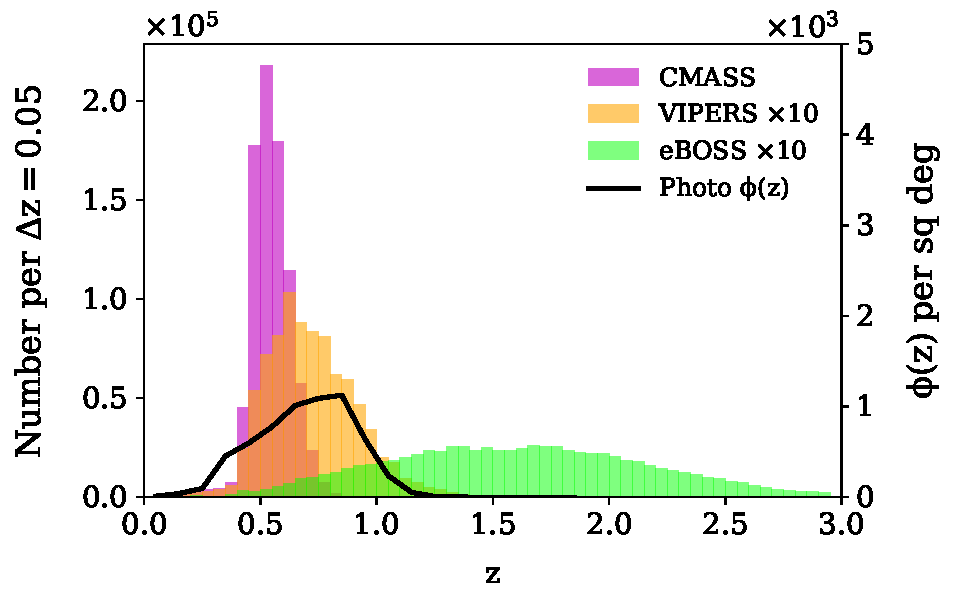
\includegraphics[width=\linewidth]{figures/spectro_overlapping_z.pdf}
\caption{Visualizing how the redshifts of the external spectroscopic catalogs (histograms) overlap with the redshift distribution of DESI LRGs selected from DECaLS, as estimated using photometric redshifts (solid line).}
\label{fig:spectro_overlap}
\end{figure}

\subsection{Results}

Following Equation~\ref{eqn:dndz_estimator}, we obtain an estimate for $dN_{\rm p}/dz$ from each cross-correlation. Bootstrap errors from $w_{\rm ps}$ are propagated to $\phi(z)$ by performing the full calculation, including normalization, with each bootstrap separately, and then determining the standard deviation in $\phi(z)$. We use a cubic B-spline to fit the combined results, where each value $\phi_i$ is weighed by the inverse of its standard deviation, $w_i = 1/\sigma_i$. 
%We apply a smoothness parameter $s$ such that $\sum_i{w_i^2 (\phi_i - g(z_i))^2} \leq s$ where $g(z)$ is the smoothed interpolation of $(z,\phi)$. 
A common rule of thumb recommends using a value of the smoothness parameter $s$ in the range $m \pm \sqrt{2m}$ where $m$ is the number of data points being fit. Based on this, we choose a value of $s = 41$, which results in 6 interior knots. In order the respect the physicality of $\phi(z) \ge 0$ for all $z$, we force any negative spline coefficients to be zero. The clustering-based $\phi(z)$ points and fit are shown in Figure~\ref{fig:clustering_dndz}, along with the photo-z derived $\phi(z)$. Unsurprisingly, the spline fit is dominated by the CMASS cross-correlations (highlighted in blue in the figure) due to the comparatively high signal-to-noise of these cross-correlations. The photo-z and clustering redshift distributions are qualitatively similar but not identical, with the clustering $\phi(z)$ having a sharper peak.

\begin{figure}
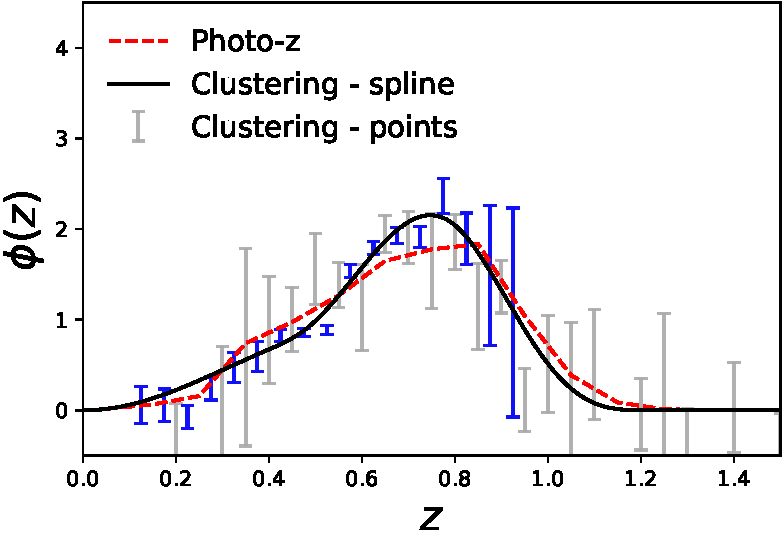
\includegraphics[width=\linewidth]{figures/clustering_dndz.pdf}
\caption{The normalized redshift distribution derived from cross-correlations with external spectroscopy (gray error bars) and resulting cubic B-spline fit (black solid line). The normalized redshift distribution derived from photo-z's is shown for comparison (red dashed line). The spline fit is dominated by the cross-correlation with CMASS galaxies (blue highlight).}
\label{fig:clustering_dndz}
\end{figure}

